\documentclass{article}

% The proposal used PRIMEarxiv.sty (Overleaf template). If it is not present, fall back to
% report/arxiv.sty from the repository, a re-creation of the same layout.
\IfFileExists{PRIMEarxiv.sty}{\usepackage{PRIMEarxiv}}{\usepackage{arxiv}}

\usepackage[utf8]{inputenc}
\usepackage[T1]{fontenc}
\usepackage{url}
\usepackage{booktabs}
\usepackage{amsfonts}
\usepackage{amsmath}
\usepackage{amssymb}
\usepackage{amsthm}
\usepackage{microtype}
\usepackage{graphicx}
\usepackage{array}
\usepackage{xcolor}
\usepackage{algorithm}
\usepackage{algpseudocode}
\usepackage{caption}
\captionsetup{font=small,labelfont=bf,skip=4pt}
\usepackage{hyperref}

\newcommand{\E}{\mathbb{E}}
\providecommand{\keywords}[1]{\par\noindent\textbf{Keywords:} #1}
\setlength{\textfloatsep}{10pt plus 2pt minus 2pt}
\setlength{\floatsep}{8pt plus 2pt minus 2pt}

\title{
Learning to Work and Save in a Shared Economy: \\
Decentralized Multi-Agent Reinforcement Learning versus the Known-Model Aiyagari Equilibrium
}
\author{}
\date{}

\hypersetup{
    pdftitle={Learning to Work and Save in a Shared Economy},
    pdfauthor={Aryan Meshram, Chaitanya Sharma, Pratik Dhakar, Saksham Chourasia},
    pdfkeywords={multi-agent reinforcement learning, heterogeneous agents, Aiyagari model, mean-field games, taxation},
}

\begin{document}

\maketitle

\vspace{-4.5em}
\begin{center}
\setlength{\tabcolsep}{22pt}
\begin{tabular}{cc}
\begin{tabular}{c}
\textbf{Aryan Meshram}\\
24110054\\
{\scriptsize\texttt{aryan.meshram@iitgn.ac.in}}
\end{tabular}
&
\begin{tabular}{c}
\textbf{Chaitanya Sharma}\\
23110072\\
{\scriptsize\texttt{chaitanya.sharma@iitgn.ac.in}}
\end{tabular}
\\[1.0em]
\begin{tabular}{c}
\textbf{Pratik Kumar Dhakar}\\
24110277\\
{\scriptsize\texttt{pratik.dhakar@iitgn.ac.in}}
\end{tabular}
&
\begin{tabular}{c}
\textbf{Saksham Chourasia}\\
24110312\\
{\scriptsize\texttt{saksham.chourasia@iitgn.ac.in}}
\end{tabular}
\end{tabular}
\end{center}

\begin{abstract}
We ask how close decentralized multi-agent reinforcement learning (MARL) gets to the exact competitive equilibrium of a heterogeneous-household economy. We build a vectorized Aiyagari-type simulator with endogenous labor, income taxes and lump-sum rebates whose resource constraint holds to $10^{-9}$, solve the \emph{same} economy exactly with a known-model benchmark (endogenous-grid dynamic programming, histogram distribution, Brent market clearing), and train shared-policy IPPO and MAPPO households in it (49 runs over five population sizes, four observation levels and seven tax regimes). Learners match equilibrium hours ($0.334$ vs.\ $0.333$) and lose only $1.3$--$1.4\%$ of consumption-equivalent welfare, against $13.5\%$ for the best constant policy. However, they under-accumulate capital by about $14\%$, produce too little wealth inequality (Gini $0.46$ vs.\ $0.55$), and are not a Nash equilibrium: an exact best response gains $0.40\%$, a gain that a PPO-trained deviator fails to find. The capital gap does not shrink like $1/N$ but sits on a learning floor of about $13\%$; observing prices reduces it, observing aggregates does not. Under income taxes, learners reproduce the signs and roughly the elasticities of the equilibrium capital and labor responses, but not the distributional response.
\end{abstract}

\keywords{Multi-agent reinforcement learning, Heterogeneous agents, Aiyagari model, Mean-field limit, Taxation, Exploitability}

%==============================================================
\section{Introduction}
%==============================================================
An economy is a very large multi-agent system. Each household chooses how much to work and save; no household controls prices, yet together their choices determine capital and labor and hence wages and interest rates, while taxes and redistribution change incentives again. Macroeconomics studies such economies with a \emph{known-model} view: in the Bewley--Huggett--Aiyagari family \cite{aiyagari1994,huggett1993} price-taking households face uninsurable income risk, and the equilibrium is computed by dynamic programming and a market-clearing fixed point; in the infinite-population limit this is a mean-field game \cite{lasry2007,light2022}, for which an RL method provably finds a regularized equilibrium \cite{xu2023}. In parallel, the AI Economist \cite{zheng2022} and TaxAI \cite{mi2024taxai} place \emph{learning} agents in economic simulators with a finite number of households, but do not compare the learned outcome with an exact solution of the same economy.

We connect the two views and ask: \emph{how close does an economy of learning households get to the known-model competitive equilibrium, and how does the gap depend on the number of households $N$, the information they observe, and the tax regime?}

\textbf{Contributions.} (i) A vectorized simulator whose aggregate resource constraint is verified to $10^{-9}$ by automated tests; (ii) an exact dynamic-programming benchmark B1 for the \emph{same} finite-state economy, cross-validated against value-function iteration; (iii) shared-policy IPPO and MAPPO households trained under five population sizes, four observation levels and seven tax regimes (49 runs); (iv) aggregate, policy, welfare, inequality and two exploitability gaps; and (v) quantified, partly negative answers to four hypotheses. Every number below is produced by the code at \url{https://github.com/AryanMeshram059/fai-group42-econ-marl}.

%==============================================================
\section{Problem Formulation}
%==============================================================
\textbf{Economy.} Households $i\in\{1,\dots,N\}$ hold assets $a_i^t\ge0$ and productivity $e_i^t$, with $\log e_i^{t+1}=\rho_e\log e_i^t+\sigma_e u_i^{t+1}$ discretized by a 7-state Rouwenhorst chain \cite{kopecky2010} that is shared by the simulator and B1 (so B1 is the exact equilibrium of the simulated economy). Each period, households simultaneously choose a saving ratio $p_i^t\in[0.001,0.99]$ and hours $h_i^t\in[0,1]$. With Cobb--Douglas production and a proportional income tax $\mathcal T(y)=\tau y$ (the HSV schedule \cite{heathcote2017} with $\xi=0$) whose revenue is rebated lump-sum with share $\psi$:
\begin{gather*}
K_t=\textstyle\sum_i a_i^t,\quad L_t=\max\big(\textstyle\sum_i e_i^th_i^t,L_{\min}\big),\quad \kappa_t=K_t/L_t,\quad
W_t=(1-\alpha)\kappa_t^{\alpha},\quad r_t=\alpha\kappa_t^{\alpha-1}-\delta,\\
y_i^t=W_te_i^th_i^t+r_ta_i^t,\qquad \nu_t=\tfrac{\psi}{N}\textstyle\sum_i\mathcal T(y_i^t),\qquad m_i^t=a_i^t+y_i^t-\mathcal T(y_i^t)+\nu_t,\\
a_i^{t+1}=p_i^tm_i^t,\qquad c_i^t=(1-p_i^t)m_i^t,\qquad
R_i^t=u(c_i^t,h_i^t)=\tfrac{(c_i^t)^{1-\theta}}{1-\theta}-\chi\tfrac{(h_i^t)^{1+\varphi}}{1+\varphi},\qquad J_i=\E\textstyle\sum_t\beta^tR_i^t .
\end{gather*}
Unrebated revenue $G_t=(1-\psi)S_t$ is government spending, and constant returns give the identity $Y_t=C_t+K_{t+1}-(1-\delta)K_t+G_t$. This is a general-sum partially observable Markov game. Households observe one of four levels: \textbf{O0} $(a_i,e_i)$; \textbf{O1} adds lagged prices $(W_{t-1},r_{t-1})$; \textbf{O2} adds $K_t/N$ and $L_{t-1}/N$; \textbf{O3} adds TaxAI-style statistics (mean wealth, lagged income and productivity) of the top-10\% and bottom-50\% wealth groups \cite{mi2024taxai}.

\textbf{Known-model benchmark B1.} Given $(\kappa,\nu)$, a price-taking household solves
\begin{equation}
V(a,e)=\max_{a'\ge0,\,h\in[0,1]}\big\{u(m(a,e,h)-a',h)+\beta\,\E[V(a',e')\mid e]\big\},
\label{eq:bellman}
\end{equation}
and the stationary equilibrium $(\kappa^\star,\nu^\star)$ satisfies $K^s/L^s=\kappa^\star$ and $\nu^\star=\psi\int\mathcal T(y)\,d\mu^\star$, where $\mu^\star$ is the stationary distribution of $(a,e)$ and $K^s=\int a\,d\mu^\star$, $L^s=\int eh^\star d\mu^\star$. As $N\to\infty$ a household's price impact vanishes, so B1 is the natural mean-field reference.

\textbf{Hypotheses.} \textbf{H1}: MARL approaches B1 in aggregates but differs in the tails of the wealth distribution. \textbf{H2}: price impact is $O(1/N)$, so the gap behaves as $\Delta(N)\approx c/N+\Delta_0$ with a learning floor $\Delta_0$. \textbf{H3}: moving from O0 to O2 reduces the gaps substantially; O3 adds less. \textbf{H4}: MARL and B1 give the same signs of the elasticities of $K$ and $L$ with respect to the net-of-tax rate $1-\tau$, possibly with different magnitudes.

%==============================================================
\section{Methodology}\label{sec:method}
%==============================================================
The system has the six components of our proposal (C1--C6), each a module of the repository.

\textbf{C1: Simulator.} $M$ economies of $N$ households are held in $[M,N]$ \texttt{float64} PyTorch tensors and advanced in one call. Safeguards are $L_{\min}=10^{-3}N$, $\kappa\in[0.5,60]$ and a consumption floor $10^{-3}$ used only inside the utility, never in the budget, so accounting stays exact. Ten automated tests simulate 16 economies for 50 periods under random actions in 8 configurations (including wealth taxes and a progressive schedule) and assert the resource identity to $10^{-9}$, the household and government budgets, and $WL+RK=Y$. \emph{Calibration:} $\alpha=0.36$, $\delta=0.06$, $\beta=0.96$, $\theta=1.5$, $\varphi=2$, $\rho_e=0.9$, $\sigma_e=0.2$; $\chi=29.70$ is set by Brent's method so that mean B1 hours equal $1/3$; initial wealth is lognormal ($\sigma=1.8$) with mean equal to B1 capital per household ($2.953$).

\textbf{C2: Benchmark B1} (Algorithm~\ref{alg:b1}). The household problem is solved with the endogenous grid method (EGM) \cite{carroll2006} extended to endogenous labor. On a 200-point grid of next-period assets $a'\in[0,400]$ (dense near zero), the Euler equation gives consumption, the intratemporal condition $\chi h^\varphi=c^{-\theta}w_e$ with $w_e=(1-\tau)We$ gives hours, and the budget $c+a'=R_aa+w_eh+\nu$, $R_a=1+(1-\tau)r$, is inverted for current assets; where the borrowing constraint binds, $a'=0$ and hours solve the constrained first-order condition by bisection. The stationary distribution uses Young's histogram method \cite{young2010} on a 1000-point grid (sparse transition matrix, power iteration to $10^{-13}$), and $\kappa^\star$ is the Brent root of $K^s/L^s-\kappa$ on a bracket that guarantees $\beta R_a<1$, with a damped fixed point for $\nu$. \emph{Validation} (6 tests): market clearing to $10^{-6}$; $r^\star<1/\beta-1$; mean (max) $\log_{10}$ Euler errors at most $-7.28$ ($-4.10$) in all seven regimes; a valid distribution; a balanced government budget; and agreement with a brute-force value-function iteration within grid resolution.

\begin{algorithm}[t]
\caption{B1: stationary equilibrium with endogenous labor (EGM + histogram + Brent)}\label{alg:b1}
\small
\begin{algorithmic}[1]
\Function{Household}{$W,r,\nu$} \Comment{EGM on the grid of next-period assets $a'_j$}
\Repeat
  \State $\tilde c_j\gets\big(\beta R_a\sum_{e'}P(e'|e)\,c(a'_j,e')^{-\theta}\big)^{-1/\theta}$;\; $\tilde h_j\gets\mathrm{clip}\big((\tilde c_j^{-\theta}w_e/\chi)^{1/\varphi},0,1\big)$
  \State $\tilde a_j\gets(\tilde c_j+a'_j-w_e\tilde h_j-\nu)/R_a$;\; $c(\cdot,e)\gets$ interpolate $(\tilde a_j,\tilde c_j)$; constrained FOC for $a<\tilde a_0$
\Until{$\max|c^{\rm new}-c|/(1+c)<10^{-10}$}
\EndFunction
\Function{Excess}{$\kappa$}
  \State $W,r\gets$ prices$(\kappa)$;\; $\nu\gets0$
  \Repeat\; policy $\gets$\Call{Household}{$W,r,\nu$};\; $\mu\gets$ Young histogram fixed point;\; $\nu\gets\frac12\nu+\frac12\psi S(\mu)$
  \Until{$|\Delta\nu|<10^{-11}$}
  \State \Return $K^s(\mu)/L^s(\mu)-\kappa$
\EndFunction
\State $\kappa^\star\gets$ Brent root of \Call{Excess}{$\cdot$};\; \Return policy, $\mu^\star$, $(\kappa^\star,\nu^\star)$
\end{algorithmic}
\end{algorithm}

\textbf{C3: Baselines.} \emph{B1-in-simulator}: every household plays the DP policy ($p=a'/m^\star$, $h=h^\star$) inside the finite-$N$ simulator, under the same dynamics and random numbers as MARL, which isolates the finite-$N$ error of the exact policy. \emph{B0}: the $\tau=0$ economy, the reference for E4. \emph{B2}: the best constant policy shared by everyone, found by a $19\times15$ grid search plus an $11\times11$ refinement ($\bar p=0.83$, $\bar h=0.35$). \emph{Random}: uniform actions.

\textbf{C4: Shared-policy IPPO and MAPPO} (Algorithm~\ref{alg:ppo}). All households share one actor, a $2\times64$ tanh MLP whose outputs give the parameters $1+\mathrm{softplus}(\cdot)$ of two Beta distributions over $(\hat p,\hat h)\in(0,1)^2$, which respect the action bounds without clipping bias. IPPO \cite{dewitt2020} uses a local critic $V(o_i)$; MAPPO \cite{yu2022} a centralized critic $V(o_i,g(s))$ with an 11-dimensional permutation-invariant summary $g$ (wealth quantiles and dispersion, mean productivity, lagged prices and labor). Training uses PPO \cite{schulman2017} with GAE \cite{schulman2016gae}:
\begin{gather*}
\delta_i^t=\tilde R_i^t+\gamma V(x_i^{t+1})-V(x_i^t),\qquad \hat A_i^t=\textstyle\sum_{l\ge0}(\gamma\lambda)^l\delta_i^{t+l},\qquad \hat G_i^t=\hat A_i^t+V_{\rm old}(x_i^t),\\
\mathcal L(\vartheta)=-\E\big[\min\big(\rho_i^t\hat A_i^t,\ \mathrm{clip}(\rho_i^t,1-\epsilon,1+\epsilon)\hat A_i^t\big)\big]+c_v\,\E\big[(V(x_i^t)-\hat G_i^t)^2\big]-c_e\,\E\big[\mathcal H(\pi_\vartheta)\big],
\end{gather*}
where $\rho_i^t$ is the probability ratio of the new and old policy and $x_i^t$ the critic input, with $\gamma=\beta=0.96$, so the RL objective \emph{is} the household's objective, and rewards scaled by $1-\beta$. Each household's advantage uses only its \emph{own} reward, so the shared update averages the households' own-policy gradients rather than the gradient of the cooperative objective: learners treat prices as part of the environment, the game stays general-sum, and the fixed point is a candidate competitive equilibrium rather than a planner's allocation. Episodes last 200 periods from a fresh lognormal draw and are bootstrapped with $V(x^{200})$ because the economic horizon is infinite. Each iteration collects $8\times10^4$ household-steps ($M=\max(1,\mathrm{round}(400/N))$ economies), followed by 4 epochs of minibatch (8192) Adam updates; learning rate $10^{-3}$ decayed linearly over 300 iterations (chosen over $3\cdot10^{-4}$ on one tuning seed: final welfare $-81.53$ vs.\ $-82.74$), clip $0.2$, $\lambda=0.95$, $c_e=10^{-3}$, $c_v=0.5$, gradient clip $0.5$.

\begin{algorithm}[t]
\caption{Shared-policy IPPO / MAPPO for $N$ households}\label{alg:ppo}
\small
\begin{algorithmic}[1]
\For{iteration $k=1,\dots,300$}
  \State reset $M$ economies (lognormal wealth, stationary productivity)
  \For{$t=0,\dots,199$} \Comment{all $M\cdot N$ households act in parallel}
    \State $o_i^t\gets$ \Call{Obs}{$s^t$, level}; sample $(\hat p_i^t,\hat h_i^t)\sim\pi_\vartheta(\cdot\mid o_i^t)$; step simulator; store $(o_i^t,u_i^t,\tilde R_i^t,\log\pi)$
  \EndFor
  \State critic input $x_i^t=o_i^t$ (IPPO) or $[o_i^t,g(s^t)]$ (MAPPO); per-household GAE, bootstrap at $t=200$
  \State 4 epochs of clipped-surrogate + value + entropy updates on minibatches pooled over households
\EndFor
\end{algorithmic}
\end{algorithm}

\textbf{C5: Evaluation.} Policies are evaluated deterministically (Beta mean) in 8 economies (2 for $N=1000$) for 500 periods from a common initial draw with \emph{common random numbers}; statistics are averaged over $t\in[300,500)$. Metrics: the aggregate gap $|\kappa-\kappa^\star|/\kappa^\star$ and the hours and saving-rate gaps; the policy gap $\sum_{a,e}\mu^\star(a,e)|p^{\rm MARL}-p^{\rm B1}|$ (likewise for $h$); the consumption-equivalent welfare loss $\lambda$ relative to B1-in-simulator, solving $(1+\lambda)^{1-\theta}U_c-U_h=\bar J^{\rm B1}$ with $U_c,U_h$ the consumption and labor parts of welfare; the wealth Gini and top-10\% share; and the convergence iteration (95\% of the welfare improvement). We use 5 seeds in E1 and 3 in E2--E4 (mean $\pm$ s.d.).

\textbf{C6: Approximate exploitability.} We freeze the learned population and measure one household's gain from deviating. (a)~\emph{DP best response}: B1's household solver at the learned economy's long-run prices, the exact best response of a price-taker; if under-saving pushes $\beta R_a\ge1$ (13 of 49 runs) no stationary optimum exists, and we use the period-0 policy of the 200-period problem. (b)~\emph{PPO best response} (E1): a single deviator warm-started from the shared actor is trained for 100 iterations in 128 economies while everyone else is frozen, keeping the best checkpoint on a validation snapshot. Both are scored from a stationary snapshot with the deviator at the 10th, 50th and 90th wealth percentiles over 200 periods; exploitability is the deviator's consumption-equivalent gain, and any positive value shows the profile is not a Nash equilibrium. As sanity checks, the DP best response gains $-0.01\%$ against B1 and $3.32\%$ against B2.

\textbf{Experiments.} E1: IPPO and MAPPO vs.\ baselines ($N=100$, O3, $\tau=0$; $2\times5$ runs). E2: $N\in\{10,30,300,1000\}$ ($4\times3$). E3: O0--O2 ($3\times3$). E4: $\tau\in\{0.1,0.2,0.3\}\times\psi\in\{0,1\}$ ($6\times3$). E2--E4 reuse the E1 IPPO runs for $N=100$, O3, $\tau=0$; 49 runs in total, about 2 hours on a 12-core laptop CPU.

%==============================================================
\section{Results}\label{sec:results}
%==============================================================
All tables and figures are generated by \texttt{scripts/make\_report\_assets.py} from the stored evaluation files. \textbf{Verification.} All 16 tests pass. Across the seven tax regimes B1 behaves as theory predicts: $\kappa^\star$ falls from $8.71$ ($\tau=0$) to $6.80$ ($\tau=0.3$, $\psi=0$) and $6.47$ ($\psi=1$), $(1-\tau)r^\star$ stays below $1/\beta-1$, and $6$--$8\%$ of households are borrowing-constrained. Executed by $N=100$ households in the simulator, the B1 policy reproduces $\kappa^\star$ to within $0.8\%$, so simulator and solver describe the same economy.

\subsection{E1: Does decentralized learning recover the equilibrium?}
\begin{table}[t]
\centering
\caption{E1 at $N=100$. W-loss: consumption-equivalent welfare loss relative to B1 in simulator. DP-BR / PPO-BR: a single deviator's consumption-equivalent gain (mean over the 10th, 50th and 90th wealth percentiles).}
\label{tab:e1}
\resizebox{\linewidth}{!}{%
\begin{tabular}{lccccccccc}
\toprule
Policy & $\kappa$ & $K/N$ & hours & $a'/m$ & Gini & Top-10\% & W-loss (\%) & DP-BR (\%) & PPO-BR (\%)\\
\midrule
B1 (theory, $N{=}\infty$) & 8.713 & 2.953 & 0.333 & 0.840 & 0.549 & 0.342 & -- & -- & --\\
B1 in simulator & 8.745 & 2.955 & 0.333 & 0.840 & 0.545 & 0.337 & 0.00 & -0.01 & --\\
B2 (best constant) & 7.985 & 2.790 & 0.350 & 0.830 & 0.196 & 0.174 & 13.53 & 3.32 & --\\
Random & 0.889 & 0.442 & 0.500 & 0.495 & 0.513 & 0.352 & 3583.29 & -- & --\\
IPPO ($n{=}5$) & 7.532 $\pm$ 0.086 & 2.520 $\pm$ 0.032 & 0.334 $\pm$ 0.002 & 0.823 $\pm$ 0.001 & 0.464 $\pm$ 0.017 & 0.297 $\pm$ 0.007 & 1.36 $\pm$ 0.10 & 0.40 $\pm$ 0.07 & -0.00 $\pm$ 0.00\\
MAPPO ($n{=}5$) & 7.563 $\pm$ 0.122 & 2.530 $\pm$ 0.052 & 0.334 $\pm$ 0.002 & 0.824 $\pm$ 0.002 & 0.454 $\pm$ 0.010 & 0.291 $\pm$ 0.010 & 1.30 $\pm$ 0.19 & 0.42 $\pm$ 0.13 & 0.02 $\pm$ 0.05\\
\bottomrule
\end{tabular}}
\end{table}

\begin{figure}[t]
\centering
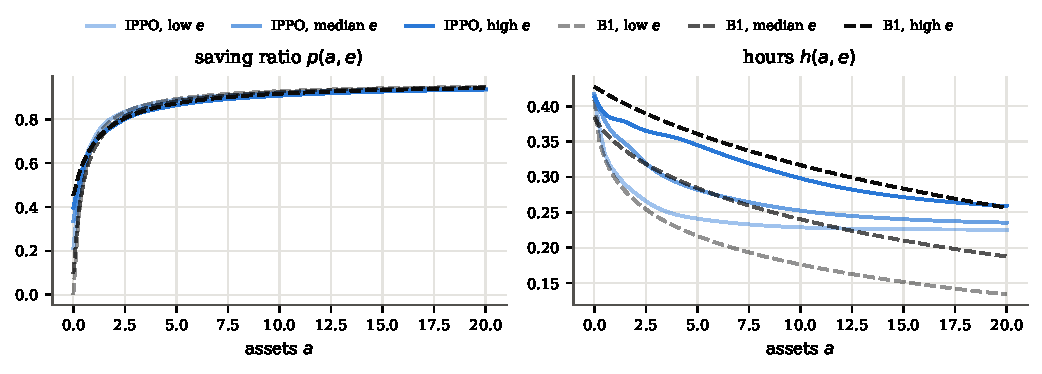
\includegraphics[width=0.86\linewidth]{figures/fig_e1_policy.pdf}
\caption{Learned (IPPO, seed 0) and B1 policy functions for low, median and high productivity.}
\label{fig:e1policy}
\end{figure}

\begin{figure}[t]
\centering
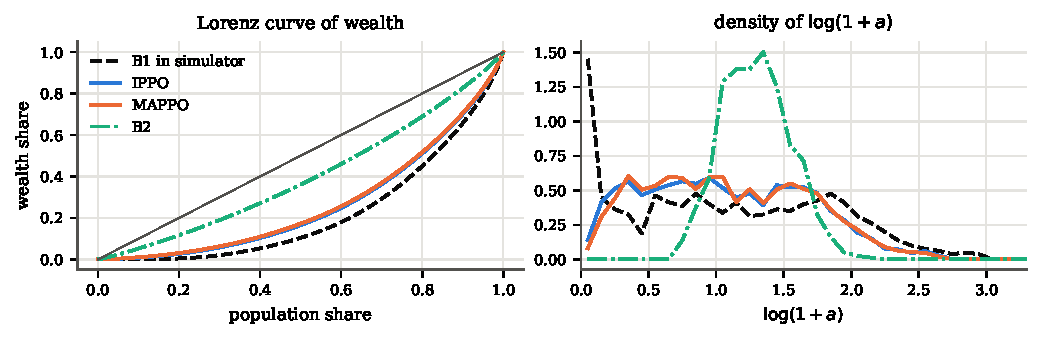
\includegraphics[width=0.86\linewidth]{figures/fig_e1_wealth.pdf}
\caption{Stationary wealth distribution at $t=500$ (pooled over seeds and evaluation economies): Lorenz curves and density of $\log(1+a)$.}
\label{fig:e1wealth}
\end{figure}

\textbf{Aggregates and welfare.} Welfare converges within 40 iterations ($3.2\times10^6$ household-steps) for both learners. The learned economy \emph{matches B1 in labor supply} (hours $0.334$ vs.\ $0.333$) but \emph{under-accumulates capital}: $\kappa=7.53\pm0.09$ (IPPO) and $7.56\pm0.12$ (MAPPO) against $\kappa^\star=8.71$, a $13.6\%$ gap, more than 30 times the finite-$N$ error of B1 itself ($0.4\%$); the interest rate is correspondingly higher ($3.9\%$ vs.\ $3.0\%$). The welfare loss is only $1.36\pm0.10\%$ (IPPO) and $1.30\pm0.19\%$ (MAPPO), whereas the best constant policy B2 loses $13.5\%$ (Table~\ref{tab:e1}): learning closes about $90\%$ of the welfare gap between a naive rule and the equilibrium.

\textbf{Policies and inequality.} The saving ratio is learned closely (policy gap $0.047$, Figure~\ref{fig:e1policy}); the error sits near the borrowing constraint, where a low-productivity learner still saves $21\%$ of cash-on-hand at $a=0$. Hours are learned less well: the wealth effect on labor is too weak, so a wealthy ($a=20$) low-productivity household works $0.23$ instead of $0.13$. The learned economy is markedly more equal (Gini $0.46$ vs.\ $0.55$; top-10\% share $0.30$ vs.\ $0.34$) because it lacks both the spike of constrained households at $a=0$ (7.4\% in B1) and the right tail (Figure~\ref{fig:e1wealth}), the regions where experience is sparse.

\textbf{Exploitability and MAPPO.} The learned profile is \emph{not} a Nash equilibrium: the DP best response gains $0.40\pm0.07\%$ (percentiles 10/50/90: $0.42/0.26/0.53\%$). The PPO best response, in contrast, finds essentially nothing ($0.00\%$ IPPO, $0.02\pm0.05\%$ MAPPO; in 9 of 10 runs no checkpoint beats the warm start), so model-free exploitability estimates can badly understate the distance to equilibrium. The centralized critic changes nothing measurable: with $N=100$ a household's value depends on the economy only through prices, which O3 already summarizes. \emph{H1: supported.}

\subsection{E2: Does the gap shrink with population size?}
\begin{table}[t]
\centering
\caption{E2: population size (IPPO, O3). B1-sim gap: finite-$N$ error of the exact policy itself. Household-steps per run: $2.4\times10^7$ ($N\le100$), $1.8\times10^7$ ($N=300$), $6\times10^7$ ($N=1000$).}
\label{tab:e2}
\resizebox{\linewidth}{!}{%
\begin{tabular}{rcccccccc}
\toprule
$N$ & $n$ & $|\Delta\kappa|/\kappa^\star$ & B1-sim gap & $p$-gap & $h$-gap & W-loss (\%) & DP-BR (\%) & time (min)\\
\midrule
10 & 3 & 0.155 $\pm$ 0.008 & 0.023 & 0.065 $\pm$ 0.006 & 0.022 $\pm$ 0.003 & -1.54 $\pm$ 0.05 & -0.33 $\pm$ 0.04 & 7.6\\
30 & 3 & 0.154 $\pm$ 0.018 & 0.054 & 0.056 $\pm$ 0.005 & 0.016 $\pm$ 0.001 & 0.78 $\pm$ 0.13 & 0.86 $\pm$ 0.24 & 9.2\\
100 & 5 & 0.136 $\pm$ 0.010 & 0.004 & 0.047 $\pm$ 0.010 & 0.014 $\pm$ 0.001 & 1.36 $\pm$ 0.10 & 0.40 $\pm$ 0.07 & 9.8\\
300 & 3 & 0.156 $\pm$ 0.027 & 0.003 & 0.062 $\pm$ 0.011 & 0.019 $\pm$ 0.001 & 2.52 $\pm$ 0.29 & 1.08 $\pm$ 0.37 & 8.9\\
1000 & 3 & 0.088 $\pm$ 0.007 & 0.005 & 0.038 $\pm$ 0.008 & 0.012 $\pm$ 0.002 & 1.47 $\pm$ 0.03 & 0.18 $\pm$ 0.03 & 22.6\\
\bottomrule
\end{tabular}}
\end{table}

\begin{figure}[t]
\centering
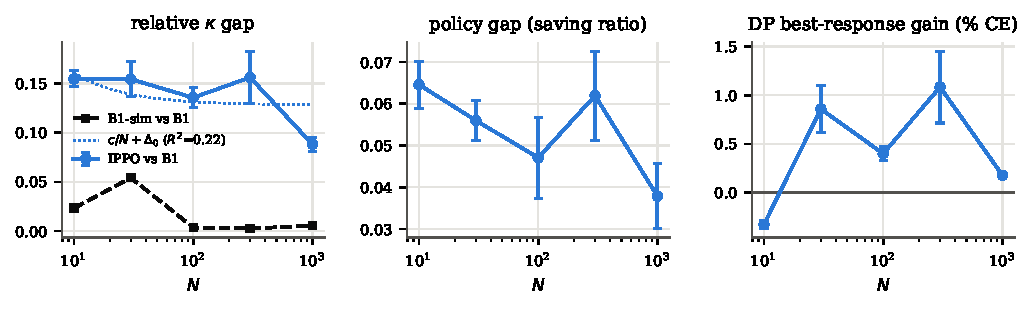
\includegraphics[width=0.95\linewidth]{figures/fig_e2_population.pdf}
\caption{E2: capital gap with the fitted $c/N+\Delta_0$ curve and the finite-$N$ error of B1 (left), saving-policy gap (middle) and DP best-response gain (right) versus $N$.}
\label{fig:e2}
\end{figure}

The \emph{learning floor dominates} (Table~\ref{tab:e2}, Figure~\ref{fig:e2}). The capital gap is $15.5$, $15.4$, $13.6$ and $15.6\%$ for $N=10,30,100,300$ and $8.8\%$ for $N=1000$; the fit gives $\Delta_0=12.8\%$ with $R^2=0.22$ (a $c/\sqrt N$ fit: $R^2=0.33$). The gap is ordered by the \emph{sample budget} rather than by $N$: the worst case ($N=300$) has the fewest household-steps and the best ($N=1000$) the most, so the improvement at $N=1000$ cannot be attributed to vanishing price impact. Price impact is visible only at $N=10$, where prices fluctuate strongly (s.d.\ of $\kappa$ under B1 $1.22$, against $0.15$ at $N=100$): the price-taking B1 policy then \emph{loses} welfare relative to the learners ($-1.54\%$) and the DP deviation computed at mean prices is worse ($-0.33\%$), while learners adapt to the actual dynamics. \emph{H2: not supported at our budget}; an $O(1/N)$ effect exists in B1 itself but is swamped by a ${\approx}13\%$ learning floor.

\subsection{E3: Does information help?}
\begin{table}[t]
\centering
\caption{E3: observation levels (IPPO, $N=100$). conv.\ iter: first evaluation reaching 95\% of the final welfare improvement.}
\label{tab:e3}
\small
\begin{tabular}{lccccccc}
\toprule
Obs. & $n$ & $|\Delta\kappa|/\kappa^\star$ & $p$-gap & $h$-gap & W-loss (\%) & DP-BR (\%) & conv. iter\\
\midrule
O0 & 3 & 0.184 $\pm$ 0.002 & 0.044 $\pm$ 0.008 & 0.012 $\pm$ 0.001 & 1.21 $\pm$ 0.08 & 0.81 $\pm$ 0.05 & 33\\
O1 & 3 & 0.158 $\pm$ 0.016 & 0.036 $\pm$ 0.006 & 0.012 $\pm$ 0.002 & 1.27 $\pm$ 0.27 & 0.49 $\pm$ 0.17 & 27\\
O2 & 3 & 0.157 $\pm$ 0.003 & 0.037 $\pm$ 0.006 & 0.012 $\pm$ 0.000 & 1.19 $\pm$ 0.06 & 0.48 $\pm$ 0.05 & 33\\
O3 & 5 & 0.136 $\pm$ 0.010 & 0.047 $\pm$ 0.010 & 0.014 $\pm$ 0.001 & 1.36 $\pm$ 0.10 & 0.40 $\pm$ 0.07 & 40\\
\bottomrule
\end{tabular}
\end{table}

Information matters for \emph{aggregates and exploitability} but not for welfare (Table~\ref{tab:e3}). Adding lagged prices (O0$\to$O1) cuts the capital gap from $18.4\%$ to $15.8\%$ and the DP best-response gain from $0.81\%$ to $0.49\%$: without prices a household cannot condition on the return to saving. Aggregates (O2) add nothing, as expected when prices are sufficient statistics for them, while the group statistics of O3 reduce the gap further to $13.6\%$. The welfare loss is flat at $1.2$--$1.4\%$, so most welfare comes from the individual state $(a,e)$ that every level observes. \emph{H3: partially supported}; prices help, but O2 adds nothing while O3 still helps, the opposite of the predicted ordering.

\subsection{E4: Do learners respond to taxes like the equilibrium?}
\begin{table}[t]
\centering
\caption{E4: income tax $\tau$ with revenue wasted ($\psi=0$) or rebated ($\psi=1$); IPPO, O3, 3 seeds ($\tau=0$: 5). B1: exact equilibrium ($K/N$, hours) and B1 in simulator (Gini, $\bar J$).}
\label{tab:e4}
\resizebox{\linewidth}{!}{%
\begin{tabular}{ccccccccc}
\toprule
$\tau$ & $\psi$ & $K/N$ MARL & $K/N$ B1 & hours MARL & hours B1 & Gini MARL & Gini B1 & $\bar J$ MARL / B1\\
\midrule
0.1 & 0 & 2.327 $\pm$ 0.012 & 2.798 & 0.336 $\pm$ 0.002 & 0.338 & 0.454 & 0.538 & -85.8 / -85.3\\
0.2 & 0 & 2.193 $\pm$ 0.048 & 2.620 & 0.342 $\pm$ 0.001 & 0.342 & 0.468 & 0.531 & -90.6 / -89.9\\
0.3 & 0 & 1.985 $\pm$ 0.034 & 2.417 & 0.351 $\pm$ 0.001 & 0.348 & 0.477 & 0.523 & -96.3 / -95.5\\
0.0 & 1 & 2.520 $\pm$ 0.032 & 2.953 & 0.334 $\pm$ 0.002 & 0.333 & 0.464 & 0.545 & -81.8 / -81.3\\
0.1 & 1 & 2.218 $\pm$ 0.048 & 2.632 & 0.320 $\pm$ 0.002 & 0.321 & 0.460 & 0.551 & -81.2 / -80.6\\
0.2 & 1 & 1.943 $\pm$ 0.015 & 2.306 & 0.307 $\pm$ 0.001 & 0.307 & 0.481 & 0.556 & -80.8 / -80.1\\
0.3 & 1 & 1.650 $\pm$ 0.029 & 1.976 & 0.291 $\pm$ 0.000 & 0.294 & 0.473 & 0.563 & -80.9 / -80.0\\
\bottomrule
\end{tabular}}
\end{table}

\begin{figure}[t]
\centering
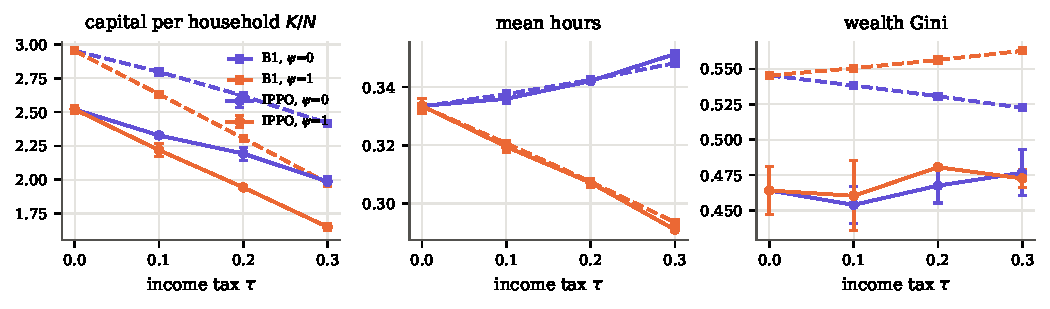
\includegraphics[width=0.95\linewidth]{figures/fig_e4_tax.pdf}
\caption{E4: capital, hours and wealth Gini versus $\tau$. Solid: IPPO (mean $\pm$ s.d.); dashed: B1.}
\label{fig:e4}
\end{figure}

The tax experiment gives the strongest agreement (Table~\ref{tab:e4}, Figure~\ref{fig:e4}). \textbf{Signs:} MARL reproduces every qualitative prediction of B1. Capital falls with $\tau$ in both regimes; hours \emph{rise} with $\tau$ when revenue is wasted (households are poorer, the income effect dominates) and \emph{fall} when it is rebated (the rebate removes the income effect). \textbf{Magnitudes:} the elasticities with respect to $1-\tau$ (least-squares slopes of logs) are close to B1's: $\varepsilon_K=0.65$ vs.\ $0.56$ and $\varepsilon_h=-0.15$ vs.\ $-0.12$ with wasted revenue, $\varepsilon_K=1.18$ vs.\ $1.13$ and $\varepsilon_h=0.38$ vs.\ $0.36$ with the rebate. Hours match B1 within $0.003$ in every regime, and the capital shortfall is a nearly constant level effect (learned $\kappa$ is $83$--$86\%$ of $\kappa^\star$ in all seven regimes) that cancels in comparative statics. \textbf{Failure:} in B1 the rebate raises the Gini ($0.545\to0.563$) and wasted revenue lowers it ($0.523$); MARL's Gini stays at $0.45$--$0.48$ with no clear trend. \emph{H4: supported} for the signs and, unexpectedly, the magnitudes of aggregate responses; \emph{not supported} for the distributional response.

%==============================================================
\section{Discussion and Conclusion}
%==============================================================
Placing MARL households and an exact equilibrium solver in the \emph{same} finite-$N$ economy turns qualitative claims that ``learners behave like an economy'' into measured gaps. Shared-policy PPO learns the intensive margins well (hours, the saving ratio away from the constraint, tax responses) and comes within $1.4\%$ of equilibrium welfare. It systematically misses precautionary wealth accumulation (a ${\approx}14\%$ capital shortfall across $N$, observation levels and tax regimes) and the shape of the wealth distribution. We conjecture that both stem from long-horizon credit assignment: the benefit of extra saving arrives decades later and only in rare bad states, so it is weak in a 200-step, $\gamma=0.96$ return; the same reason explains why model-free exploitability (PPO-BR $\approx0$) underestimates the model-based one (DP-BR $0.4\%$). The success criteria of the proposal (a simulator passing the accounting test, a validated B1 solver, quantified answers to H1--H4) are met, and the stretch goals MAPPO, E3 and E4 were completed.

\textbf{Limitations.} One learning rate tuned on one seed and 300 iterations per run; sample budgets differ across $N$, which confounds E2; E2--E4 use 3 rather than 5 seeds; DP best responses assume constant prices, which is inaccurate at $N=10$; only proportional taxes ($\xi=0$) were run, and the ablations A1--A4 were not. \textbf{Future work:} longer training or horizon curricula to test whether the capital floor is a budget effect, recurrent policies, progressive taxation, and a learning government on top of the household equilibrium, as in TaxAI.

\textbf{Code availability.} \url{https://github.com/AryanMeshram059/fai-group42-econ-marl} contains all code, the 49 trained models and their logs. The pipeline \texttt{pytest tests} $\rightarrow$ \texttt{calibrate.py} $\rightarrow$ \texttt{run\_benchmarks.py} $\rightarrow$ \texttt{run\_experiments.py} $\rightarrow$ \texttt{make\_report\_assets.py} regenerates every table and figure, from the stored models without retraining.

%==============================================================
\section{Contribution}
%==============================================================
The work was divided into four equal shares, each consisting of one system component, one experiment and the matching parts of the report. The \emph{Status} column records whether the assigned task was delivered.

\begin{table}[h]
\centering
\caption{Task assignment and completion.}
\label{tab:contrib}
\small
\begin{tabular}{@{}p{2.6cm}p{11.2cm}p{1.5cm}@{}}
\toprule
\textbf{Member} & \textbf{Assigned tasks} & \textbf{Status} \\
\midrule
Aryan Meshram & \textbf{C1 Environment:} vectorized simulator (prices, taxes, rebate, safeguards), Rouwenhorst process, accounting-identity tests, calibration of $\chi$ and initial wealth. \textbf{E2:} population-size runs and the $c/N+\Delta_0$ fit. \textbf{Report:} problem formulation, C1 and E2. & Fulfilled \\
Chaitanya Sharma & \textbf{C2--C3 Benchmarks:} EGM solver with endogenous labor, histogram distribution, Brent equilibrium, VFI cross-check and B1 tests; baselines B0, B1-in-simulator, B2, Random. \textbf{E4:} B1 for the seven tax regimes, tax runs and elasticities. \textbf{Report:} C2--C3 and E4. & Fulfilled \\
Pratik Kumar Dhakar & \textbf{C4 Learning:} shared-policy IPPO and MAPPO with Beta policies, observation levels O0--O3, MAPPO global summary, learning-rate tuning, parallel multi-seed training of the 49-run grid. \textbf{E3:} observation-level runs. \textbf{Report:} C4 and E3. & Fulfilled \\
Saksham Chourasia & \textbf{C5--C6 Evaluation:} aggregate, policy, welfare and inequality metrics, DP and PPO best-response exploitability, report-asset script. \textbf{E1:} IPPO vs.\ MAPPO vs.\ baselines. \textbf{Report:} C5--C6, E1 and integration of the final report. & Fulfilled \\
\bottomrule
\end{tabular}
\end{table}

Items of the proposal not completed are not tied to a single member: the ablations A1--A4 (``if time permits'') were not run, and E2--E4 use 3 rather than 5 seeds because of the compute budget.

%==============================================================
% References
%==============================================================
{\small
\begin{thebibliography}{99}\setlength{\itemsep}{0pt}
\bibitem{mi2024taxai} Q.~Mi, S.~Xia, Y.~Song, H.~Zhang, S.~Zhu, and J.~Wang. {TaxAI}: A dynamic economic simulator and benchmark for multi-agent reinforcement learning. In \emph{Proc.\ AAMAS}, pages 1390--1398, 2024.
\bibitem{aiyagari1994} S.~R. Aiyagari. Uninsured idiosyncratic risk and aggregate saving. \emph{Quarterly Journal of Economics}, 109(3):659--684, 1994.
\bibitem{huggett1993} M.~Huggett. The risk-free rate in heterogeneous-agent incomplete-insurance economies. \emph{Journal of Economic Dynamics and Control}, 17(5--6):953--969, 1993.
\bibitem{heathcote2017} J.~Heathcote, K.~Storesletten, and G.~L. Violante. Optimal tax progressivity: An analytical framework. \emph{Quarterly Journal of Economics}, 132(4):1693--1754, 2017.
\bibitem{xu2023} R.~Xu, Y.~Min, T.~Wang, Z.~Wang, M.~I. Jordan, and Z.~Yang. Finding regularized competitive equilibria of heterogeneous agent macroeconomic models via reinforcement learning. In \emph{Proc.\ AISTATS}, PMLR 206, 2023.
\bibitem{lasry2007} J.-M. Lasry and P.-L. Lions. Mean field games. \emph{Japanese Journal of Mathematics}, 2(1):229--260, 2007.
\bibitem{light2022} B.~Light and G.~Y. Weintraub. Mean field equilibrium: Uniqueness, existence, and comparative statics. \emph{Operations Research}, 70(1):585--605, 2022.
\bibitem{zheng2022} S.~Zheng et~al. The {AI} {E}conomist: Taxation policy design via two-level deep multiagent reinforcement learning. \emph{Science Advances}, 8(18), 2022.
\bibitem{yu2022} C.~Yu et~al. The surprising effectiveness of {PPO} in cooperative multi-agent games. In \emph{NeurIPS}, volume~35, 2022.
\bibitem{dewitt2020} C.~Schroeder de~Witt et~al. Is independent learning all you need in the {StarCraft} multi-agent challenge? arXiv:2011.09533, 2020.
\bibitem{schulman2017} J.~Schulman, F.~Wolski, P.~Dhariwal, A.~Radford, and O.~Klimov. Proximal policy optimization algorithms. arXiv:1707.06347, 2017.
\bibitem{kopecky2010} K.~A. Kopecky and R.~M.~H. Suen. Finite state {M}arkov-chain approximations to highly persistent processes. \emph{Review of Economic Dynamics}, 13(3):701--714, 2010.
\bibitem{carroll2006} C.~D. Carroll. The method of endogenous gridpoints for solving dynamic stochastic optimization problems. \emph{Economics Letters}, 91(3):312--320, 2006.
\bibitem{young2010} E.~R. Young. Solving the incomplete markets model with aggregate uncertainty using the {K}rusell--{S}mith algorithm and non-stochastic simulations. \emph{Journal of Economic Dynamics and Control}, 34(1):36--41, 2010.
\bibitem{schulman2016gae} J.~Schulman, P.~Moritz, S.~Levine, M.~I. Jordan, and P.~Abbeel. High-dimensional continuous control using generalized advantage estimation. In \emph{Proc.\ ICLR}, 2016.
\end{thebibliography}
}

\end{document}
